
% ===============================================
% MATH ΙΙ: Multivariable calculus           Spring 2019
% ===============================================

\documentclass{article}

\usepackage[margin=0.75in]{geometry}
\usepackage{amsmath,amsthm,amssymb,hyperref}
\usepackage[english,greek]{babel}
\usepackage[utf8x]{inputenc}

\usepackage{graphicx}
\
\newcommand{\R}{\mathbf{R}}  
\newcommand{\Z}{\mathbf{Z}}
\newcommand{\N}{\mathbf{N}}
\newcommand{\Q}{\mathbf{Q}}

\newenvironment{theorem}[2][Theorem]{\begin{trivlist}
\item[\hskip \labelsep {\bfseries #1}\hskip \labelsep {\bfseries #2.}]}{\end{trivlist}}
\newenvironment{lemma}[2][Lemma]{\begin{trivlist}
\item[\hskip \labelsep {\bfseries #1}\hskip \labelsep {\bfseries #2.}]}{\end{trivlist}}
\newenvironment{claim}[2][Claim]{\begin{trivlist}
\item[\hskip \labelsep {\bfseries #1}\hskip \labelsep {\bfseries #2.}]}{\end{trivlist}}
\newenvironment{problem}[2][Problem]{\begin{trivlist}
\item[\hskip \labelsep {\bfseries #1}\hskip \labelsep {\bfseries #2.}]}{\end{trivlist}}
\newenvironment{proposition}[2][Proposition]{\begin{trivlist}
\item[\hskip \labelsep {\bfseries #1}\hskip \labelsep {\bfseries #2.}]}{\end{trivlist}}
\newenvironment{corollary}[2][Corollary]{\begin{trivlist}
\item[\hskip \labelsep {\bfseries #1}\hskip \labelsep {\bfseries #2.}]}{\end{trivlist}}

\newenvironment{solution}{\begin{proof}[Solution]}{\end{proof}}

\begin{document}

% ------------------------------------------ %
%                 START HERE             %
% ------------------------------------------ %

\begin{figure}[h!]
  
\includegraphics[width=0.1\textwidth]{logo_uop.png}
  % \caption{}
  \label{fig:logo}
\end{figure}

{ΜΑΘ-ΙΙ
\hfill  2η Σειρά Ασκήσεων

\vspace{0.05in}

% -----------------------------------------------------
% The "enumerate" environment allows for automatic problem numbering.
% To make the number for the next problem, type " \item ". 
% To make sub-problems such as (a), (b), etc., use an "enumerate" within an "enumerate."
% Use \selectlanguage{english} to switch to english and \selectlanguage{greek} to 
% switch to greek
% -----------------------------------------------------

\begin{enumerate}
% -----------------------------------------------------
% First problem
% -----------------------------------------------------

\item  Να υπολογιστούν τα διπλά ολοκληρώματα πάνω στο ορθογώνιο \selectlanguage {english}R\selectlanguage{greek}

\begin{enumerate}{}

\item $$\iint _{R} xy\sqrt{1 + x^2 + y^2}dxdy,\;R:0\leq x\leq 1,\; 0\leq y \leq 1$$ \\
Λύση:
\begin{eqnarray*}
I &=& \iint _{R} xy\sqrt{1 + x^2 + y^2}dxdy \\
& = & \int _{0} ^{1} dy \int _{0}^{1}dx\;xy\sqrt{1 + x^2 + y^2} \\
& = & \int _{0} ^{1} dy \; y\left[ \frac{1}{3}(1 + x^2 + y^2)^{\frac{3}{2}}\right]^{x=1}_{x=0} \\
& = & \frac{1}{3}\left( \int _0 ^1 y(2+y^2)^{\frac{3}{2}} dy - \int _0 ^1 y(1+y^2)^{\frac{3}{2}} dy \right) \\
& = & \frac{1}{3} \left[\frac{1}{5}(2 + y^2)^{\frac{5}{2} \right]^1_0 - \left[\frac{1}{5}(1 + y^2)^{\frac{5}{2}} \right]^1_0 \\
& = & \frac{9\sqrt{3} - 8\sqrt{2} +1}{15}
\end{eqnarray*}

\item $$\iint _{R} \frac{1}{(x+y+1)^3}dxdy,\;R:0\leq x\leq 2,\; 0\leq y \leq 1$$ \\
Λύση:
\begin{eqnarray*}
I &=& \iint _{R} \frac{1}{(x+y+1)^3}dxdy \\
& = & \int _{0} ^{1} dy \int _{0}^{2} dx \frac{1}{(x+y+1)^3} \\
& = & \int _{0} ^{1} dy \left[ -\frac{1}{2(x+y+1)^2]} \right]^2_0 \\
& = & \int _{0} ^{1} -\frac{1}{2(y+3)^2} + \frac{1}{2(y+1)^2} dy\\
& = & \left[ \frac{1}{2(y+3)} -\frac{1}{2(y+1)]} \right]^1_0 \\
& = & \frac{5}{24}
\end{eqnarray*}

\item $$\iint _{R} xsin(xy)dxdy,\;R:0\leq x\leq 1,\; \pi\leq y \leq 2\pi$$ \\
Λύση:
\begin{eqnarray*}
I &=& \iint _{R} xsin(xy)dxdy \\
& = & \int _{\pi} ^{2\pi} dy \int _{0}^{1} dx xysin(xy) \\
& = & \int _{\pi} ^{2\pi} dy \left[ -\frac{1}{y}xcos(xy) + \frac{1}{y^2}sin(xy) \right]^1_0 \\
& = & \int _{\pi} ^{2\pi} -\frac{1}{y}0cos(xy) + \frac{1}{y^2}sin(0y) + \frac{1}{y}cos(y) -\frac{1}{y^2}sin(y) dy\\
& = &  \int _{\pi} ^{2\pi} \frac{1}{y}cos(y) -\frac{1}{y^2}sin(y) dy\\
& = & \left[ \frac{1}{y}sin(y) \right]^{2\pi}_{\pi} \\
& = & 0
\end{eqnarray*}

\item $$\iint _{R} (2x-3y^2)dxdy,\;R:-1\leq x\leq 1,\; 0\leq y \leq 2$$ \\
Λύση:
\begin{eqnarray*}
I &=& \iint _{R} (2x-3y^2)dxdy \\
& = & \int _{0} ^{2} dy \int_{-1}^{1} dx (2x-3y^2) \\
& = & \int _{0} ^{2} \left[ x^2-3y^2x \right]^1_{-1} dy\\
& = & \int _{0} ^{2} 1-3y^2-1-3y^2 dy\\
& = & \int _{0} ^{2} -6y^2 dy\\
& = & \left[ -2y^3 \right]^2_0\\
& = & -16
\end{eqnarray*}

\item $$\iint _{R} xcos(x^2+y)dxdy,\;R:-\sqrt{\pi}\leq x\leq 0,\; 0\leq y \leq \pi$$ \\
Λύση:
\begin{eqnarray*}
I &=& \iint _{R} xcos(x^2+y) dxdy \\
& = & \int _{0} ^{\pi} dy \int_{-\sqrt{\pi}}^{0} dx xcos(x^2+y) \\
& = & \int _{0} ^{\pi} \left[ \frac{1}{2}sin(x^2+y) \right]^0_{-\sqrt{\pi}} dy\\
& = & \int _{0} ^{\pi} \frac{1}{2}sin(y)-\frac{1}{2}sin(\pi+y) dy\\
& = & \int _{0} ^{\pi} \frac{1}{2}sin(y)+\frac{1}{2}sin(y) dy\\
& = & \left[ -cos(y) \right]^{\pi}_{0}\\
& = & 2
\end{eqnarray*}

\item $$\iint _{R} x^2ye^{xy}dxdy,\;R:0\leq x\leq 1,\; 0\leq y \leq 2$$ \\
Λύση:
\begin{eqnarray*}
I &=& \iint _{R} x^2ye^{xy} dxdy \\
& = & \int _{0} ^{2} dy \int_{0}^{1} dx x^2ye^{xy} \\
Use\ factorial\ integration\ two\ times. \selectlanguage{english} & = & \int _{0} ^{2} dy\ y\int_{0}^{1} dx x^2e^{xy} \\
Evaluate\ the\ integral\ of\ each\ term. \selectlanguage{english} & = & \int _{0} ^{2} e^y-\frac{2e^y}{y}+\frac{2e^y-2}{y^2} dy \\
& = & 2
\end{eqnarray*}

\end{enumerate}

% -----------------------------------------------------
% Second problem
% -----------------------------------------------------

\item  Γράψτε τα ακόλουθα ολοκληρώματα σαν γινόμενο απλών ολοκληρωμάτων και να υπολογιστούν. \selectlanguage{greek}

\begin{enumerate}{}

\item $$\iint _{R} \frac{x^2}{1+y^2} dxdy,\;R:0\leq x\leq 1,\; 0\leq y \leq 1$$ \\
Λύση:
\begin{eqnarray*}
I &=& \iint _{R}\frac{x^2}{1+y^2} dxdy \\
& = & \int _{0} ^{1} dy \frac{1}{1+y^2} \int_{0}^{1} dx x^2 \\
& = & \left[ tan^{-1}(y) \right]^1_0*\left[ \frac{x^3}{3} \right]^1_0\\
& = & \frac{\pi}{12}
\end{eqnarray*}

\item $$\iint _{R} \frac{x}{y} dxdy,\;R:0\leq x\leq 2,\; 1\leq y \leq e$$ \\
Λύση:
\begin{eqnarray*}
I &=& \iint _{R}\frac{x}{y} dxdy \\
& = & \int _{1} ^{e} dy \frac{1}{y} \int_{0}^{2} x dx \\
& = & \left[ ln|y| \right]^e_1*\left[ \frac{x^2}{2} \right]^2_0\\
& = & 2
\end{eqnarray*}

\item $$\iint _{R} e^{x-y}dxdy,\;R:-1\leq x\leq 1,\; -1\leq y \leq 1$$ \\
Λύση:
\begin{eqnarray*}
I &=& \iint _{R}e^{x-y} dxdy \\
& = & \int _{-1} ^{1} dy e^{-y} \int_{-1}^{1} e^x dx \\
& = & \left[ -e^{-y} \right]^1_{-1}*\left[ e^x\right]^1_{-1}\\
& = & -2+e^2+e^{-2}
\end{eqnarray*}

\item $$\iint _{R} xy(x^2+y^2) dxdy,\;R:0\leq x\leq 1,\; 0\leq y \leq 1$$ \\
Λύση:
\begin{eqnarray*}
I &=& \iint _{R}xy(x^2+y^2) dxdy \\
& = & \int _{0} ^{1} \int _{0} ^{1} x^3y+xy^3 dxdy\\
& = & \int _{0} ^{1} xy^3 dy \int _{0} ^{1} x^3y dx\\
& = & \int _{0} ^{1} x dy \int _{0} ^{1} y^3dy + \int _{0} ^{1}x^3 dx \int _{0} ^{1} y dy\\
& = & \left[ \frac{x^2}{2} \right]^1_0\left[ \frac{y^4}{4} \right]^1_0+\left[ \frac{x^4}{4}\right]^1_0\left[ \frac{y^2}{2}\right]^1_0\\
& = \frac{1}{4}
\end{eqnarray*}

\item $$\iint _{R} cos(x+y) dxdy,\;R:-\frac{\pi}{4}\leq x\leq \frac{\pi}{4} ,\; 0\leq y\leq\frac{\pi}{4}$$\\
Λύση:
\begin{eqnarray*}
I &=& \iint _{R}cos(x+y) dxdy \\
& = & \int _{0} ^{\frac{\pi}{4}} \int _{-{\frac{\pi}{4}}} ^{{ \frac{\pi}{4}}} cos(x+y) dxdy\\
& = & \int _{0} ^{\frac{\pi}{4}} \int _{-{\frac{\pi}{4}}} ^{{ \frac{\pi}{4}}} cosxcosy-sinxsinydxdy\\
& = & \int _{0} ^{\frac{\pi}{4}} \int _{-{\frac{\pi}{4}}} ^{{ \frac{\pi}{4}}} cosxcosydxdy-\int _{0} ^{\frac{\pi}{4}} \int _{-{\frac{\pi}{4}}} ^{{ \frac{\pi}{4}}} sinxsinydxdy\\
& = & \int _{0} ^{\frac{\pi}{4}} cosxdx \int _{-{\frac{\pi}{4}}} ^{{ \frac{\pi}{4}}} cosydy-\int _{0} ^{\frac{\pi}{4}}sinxdx \int _{-{\frac{\pi}{4}}} ^{{ \frac{\pi}{4}}} sinydy\\
& = & \left[ sinx \right]^{\frac{\pi}{4}}_0\left[ siny \right]^{\frac{\pi}{4}}_{-{\frac{\pi}{4}}}-\left[ -cosx\right]^{\frac{\pi}{4}}_0\left[ -cosy\right]^{\frac{\pi}{4}}_{-{\frac{\pi}{4}}}\\
& = & 1
\end{eqnarray*}

\item $$\iint _{R} xyln\frac{x}{y} dxdy,\;R:1\leq x\leq e ,\; 1\leq y\leq\ 2 $$\\
Λύση:
\begin{eqnarray*}
I &=& \iint _{R}xyln\frac{x}{y} dxdy \\
& = & \int _{1} ^{2} \int _{1} ^{e} xylnx-xylny dxdy\\
& = & \int _{1} ^{2}ydy \int _{1}  ^{e}xlnxdx -\int _{1} ^{2}ylnydy \int _{1}  ^{e}xdx\\
& = & \left[ \frac{y^2}{2} \right]^2_1*\left[ \frac{x^2}{2}lnx-\frac{x^2}{4}\right]^e_1- \left[ \frac{y^2}{2}lny-\frac{y^2}{4} \right]^2_1*\left[ \frac{x^2}{2}\right]^e_1\\
& = & e^2(\frac{3}{4}-ln2)+ln2\\
\end{eqnarray*}

\end{enumerate}


% -----------------------------------------------------
% Third problem
% -----------------------------------------------------

\item  Γράψτε αναλυτικά την έκφραση Ι και να σχεδιάσεται τα χωρία ολοκλήρωσης, I &=& \iint f(x,y) dxdy.\selectlanguage {greek}

\begin{enumerate}{}

\item $$ x=0,\ y=0,\ x^2+y^2=25,\ 0\leq x,\; 0\leq y $$\\
Λύση:
\begin{eqnarray*}
Solve\ x^2+y^2=25\ for\ y. \selectlanguage{english}\\
\\x>0\\
y>0\\
y=\sqrt{25-x^2}\\
x>5\\
I &=& \int _{0} ^{5} ( \int _{0} ^{\sqrt{25-x^2}} f(x,y)\ dy )\ dx\\

\begin{figure}[h!]
  \centering
  \includegraphics[width=0.3\textwidth]{y=sqrt{25-x^2}.png}
\end{figure}

\end{eqnarray*}


\item $$ y=\frac{1}{x},\ y=\sqrt{x},\ x=2 $$\\
Λύση:
\begin{eqnarray*}
x=2\\
\\
y=y\\
1/x=\sqrt{x}\\
x=1\\
\\
I &=& \int _{1} ^{2} ( \int _{\frac{1}{x}} ^{\sqrt{x}} f(x,y)\ dy )\ dx\\

\begin{figure}[h!]
  \centering
  \includegraphics[width=0.3\textwidth]{y=frac{1}{2},y=sqrt{x}.png}
\end{figure}

\end{eqnarray*}


\item $$ x^2+y=2,\ y^3=x^2,\ x=0 $$\\
Λύση:
\begin{eqnarray*}
x=0\\
\\
y^3=x^2\\
y=x^\frac{2}{3}\\
\\
x^2+y=2\\
y=2-x^2\\
\\
y=y\\
x^\frac{2}{3}=2-x^2,\ x>0\ \\
x=1\\
\\
I &=& \int _{0} ^{1} ( \int _{x^\frac{2}{3}} ^{2-x^2} f(x,y)\ dy )\ dx\\

\begin{figure}[h!]
  \centering
  \includegraphics[width=0.3\textwidth]{y=x^(frac{2}{3}),y=2-x^2.png}
\end{figure}

\end{eqnarray*}

\end{enumerate}


% -----------------------------------------------------
% Fourth problem
% -----------------------------------------------------

\item  Αντιστρέψτε τη σειρά ολοκλήρωσης στα ακόλουθα ολοκληρώματα και να σχεδιάσεται τα χωρία ολοκλήρωσης.\selectlanguage {greek}

\begin{enumerate}{}

\item $$ \int _{0} ^{1} dx \int _{0} ^{lnx} 1\ dy $$\\
Λύση:
\begin{eqnarray*}
\;R:0\leq x\leq 1 ,\; 0\leq y\leq\ lnx\\
\;R:e\leq x\leq e^y ,\; 0\leq y\leq\ 1\\
I &=& \int _{0} ^{-\infty} dy \int _{0} ^{e^y} dx \\
& = & \int _{0} ^{-\infty} e^y dy \\
& = & -1
\end{eqnarray*}

\begin{eqnarray*}
I &=& \int _{0} ^{1} lnx\ dx \int _{0} ^{e^y} dx \\
& = & \left[ (x*lnx)-x \right]^1_0\\
& = & -1-\left[(x*lnx)-x) \right]^____x=0\\
& = & -1\\
(\lim_{x\to 0} ((x*lnx)-x) = 0)\\

\begin{figure}[h!]
  \centering
  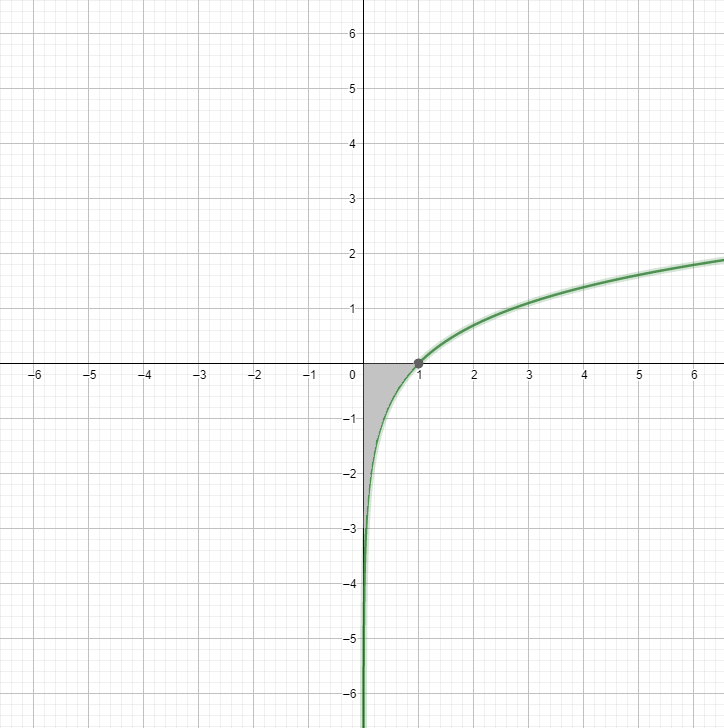
\includegraphics[width=0.3\textwidth]{y=lnx.png}
\end{figure}

\end{eqnarray*}


\item $$ \int _{0} ^{1} dy \int _{y^2} ^{\sqrt{y}} 1\ dx $$\\
Λύση:
\begin{eqnarray*}
I &=& \int _{0} ^{1} dx \int _{x^2} ^{\sqrt{x}} 1\ dy \\
& = & \int _{0} ^{1} \left[ y \right]^{\sqrt{x}}_{x^2}\ dx\\
& = & \int _{0} ^{1} \sqrt{x}-x^2\ dx \\
& = & \left[ \frac{2}{3}x^{\frac{3}{2}}-\frac{x^3}{3} \right]^{1}_{0}\\
& = & \frac{1}{3}


\begin{figure}[h!]
  \centering
  \includegraphics[width=0.2\textwidth]{sqrt{x},y=x^2.png}}
\end{figure}

\end{eqnarray*}


\item $$ \int _{0} ^{\pi/2} dx \int _{sinx} ^{2} 1\ dy $$\\
Λύση:
\begin{eqnarray*}
I &=& \int _{0} ^{\pi/2} dx \int _{sinx} ^{1} 1\ dy + \int _{0} ^{\pi/2} dx \int _{1} ^{2} 1\ dy \\
& = & \int _{0} ^{1} dy \int _{0} ^{arcsinx} 1\ dx + \int _{1} ^{2} dy \int _{0} ^{\pi/2} 1\ dx \\
& = & \int _{0} ^{1} \left[x \right]^{arcsinx}_{0} dy + \int _{1} ^{2} \left[x \right]^{\pi/2}_{0} dy \\
& = & \int _{0} ^{1} arcsiny\ dy + \int _{1} ^{2} \pi/2\ dy \\
& = & \left[y*arcsiny + (1-y^2)^{\frac{1}{2}} \right]^{1}_{0} + \left[\frac{\pi}{2}*x \right]^{2}_{1} \\
& = & \pi-1

\begin{figure}[h!]
  \centering
  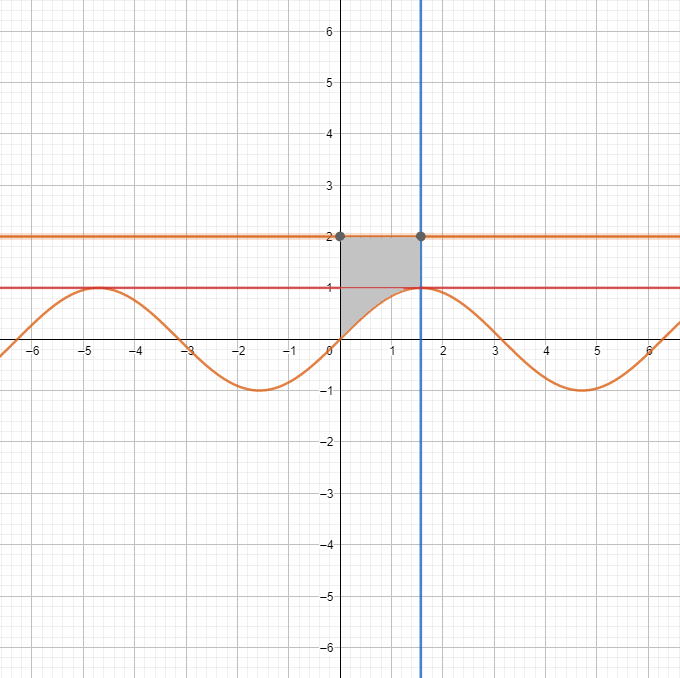
\includegraphics[width=0.3\textwidth]{y=sin(x),y=1,y=2,x=pi2.png}
\end{figure}

\end{eqnarray*}

\end{enumerate}


% -----------------------------------------------------
% fifth problem
% -----------------------------------------------------
\item  Να υπολογιστούν τα ακόλουθα ολοκληρώματα και να σχεδιάσετε τα χωρία ολοκλήρωσης.\selectlanguage {greek}

\begin{enumerate}{}
\item $$ D:  y = -\sqrt{x}, y = \frac{1}{x}, x = 1, x = 2 $$\\
Λύση :
\begin{eqnarray*}
I &=& \int _{1} ^{2} dx \int _{-\sqrt{x}} ^{\frac{1}{x}} x^2y dy\\
& = & \int_{1} ^{2}\left[x^2\frac{y^2}{2}\right]^{\frac{1}{x}}_{-\sqrt{x}} dx\\
& = & \int _{1}^{2}(x^2\frac{1}{2x^2}-x^2\frac{(-\sqrt{x})^2}{2}) dx\\
& = & \int _{1} ^{2}(\frac{1}{2}-\frac{x^3}{2}) dx \\
& = & \left[\frac{1}{2}x-\frac{x^4}{8}\right]^{2}_{1}\\
& = & -\frac{11}{8}
\end{enumerate}
\begin{figure}[h!]
  \centering
  \includegraphics[width=0.2\textwidth]{y=-sqrt{x},y=frac{1}{x},x=1,x=2.png}
\end{figure}
\item $$ D: y = -x^2+4, y =3\sqrt{x},y=0 $$\\
Λύση :
\begin{eqnarray*}
I &=& \int_{0}^{1}\int_{3\sqrt{x}}^{-x^2+4}xydydx\\
& = & \int_{0}^{1}\left[x\frac{y^2}{2}\right]_{3\sqrt{x}}^{-x^2+4}dx\\
& = & \int_{0}^{1}(-\frac{9x^2}{2}+\frac{x^5-8x^3+16x}{2})dx\\
& = & \frac{1}{2}\left[\frac{x^6}{6}-\frac{8x^4}{4}-\frac{9x^3}{3}+\frac{16x^2}{2}\right]_{0}^{1}\\
& = & \frac{19}{12}\\
\end{enumerate}
\begin{figure}[h!]
  \centering
  \includegraphics[width=0.2\textwidth]{y=-x^2+4,y=3sqrt{x},y=0.png}
\end{figure}
\item $$ D: y = x^2, y^2 = x, x = 1, x = 2 $$\\
Λύση :
\begin{eqnarray*}
I &=& \int _{0} ^{1} dx \int _{x^2}^{\sqrt{x}}(x^2+y) dy \\
& = & \int_{0} ^{1}\left[x^2y+\frac{y^2}{2}\right]^{\sqrt{x}}_{x^2}dx\\
& = & \int _{0}^{1}(x^2\sqrt{x}+\frac{x}{2}-x^4-\frac{x^4}{2}) dx\\
& = & \int _{0} ^{1}(x^\frac{5}{2}+\frac{x}{2}-3\frac{x^4}{2}) dx \\
& = & \left[\frac{2}{7}x^\frac{7}{2}+\frac{x^2}{4}-3\frac{x^5}{10}\right]^{1}_{0}\\
& = & \frac{33}{140}
\end{enumerate}
\begin{figure}[h!]
  \centering
  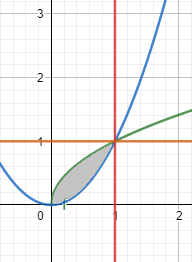
\includegraphics[width=0.2\textwidth]{y=x^2,y^2=x.png}
\end{figure}
\item $$ D: y = \frac{1}{x}, y = x, x = 2 $$\\
Λύση :
\begin{eqnarray*}
I &=& \int _{1} ^{2} dx \int _{x}^{\frac{1}{x}}\frac{x^2}{y^2} dy \\
& = & \int_{1} ^{2}\left[-\frac{x^2}{y}\right]^{\frac{1}{x}}_{x}dx\\
& = & \int _{1}^{2}(-\frac{x^2}{\frac{1}{x}}+\frac{x^2}{x})dx\\
& = & \int _{1} ^{2}(-x^3+x) dx \\
& = & \left[-\frac{x^4}{4}+\frac{x^2}{2}\right]^{2}_{1}\\
& = & \frac{9}{4}
\end{enumerate}
\begin{figure}[h!]
  \centering
  \includegraphics[width=0.2\textwidth]{y=frac{1}{x},y=x,x=2.png}
\end{figure}
\\\\\\\\\item $$ D: y = x^2, y = 4-x^2 $$\\
Λύση :
\begin{eqnarray*}
I &=& \int _{-\sqrt{2}} ^{\sqrt{2}} dx \int_{x^2}^{4-x^2} 1 dy \\
& = & \int_{-\sqrt{2}} ^{\sqrt{2}}\left[y\right]^{x^2}_{4-x}dx\\
& = & \int _{-\sqrt{2}}^{\sqrt{2}}(2x^2-4)dx\\
& = & \left[2\frac{x^3}{3}-4x\right]^{\sqrt{2}}_{-\sqrt{2}}\\
& = & \frac{16\sqrt{2}}{3}
\end{enumerate}
\begin{figure}[h!]
  \centering
  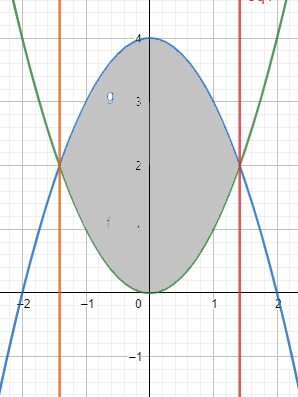
\includegraphics[width=0.2\textwidth]{y=x^2,y=4-x^2.png}
\end{figure}
\item $$ D: y^2 = x+2, y = -x, x=2 $$\\
Λύση :
\begin{eqnarray*}
I & = & \int_{-1}^{2}\int_{-x}^{\sqrt{x+2}}2xdydx\\
& = & \int_{-1}^{2}\left[2xy\right]_{-x}^{\sqrt{x+2}}dx\\
& = & \left[\frac{10x^3+20x(x+2)^\frac{3}{2}-8(x+2)^\frac{5}{2}}{15}\right]_{-1}^{2}\\
& = & \frac{182}{15}
\end{enumerate}
\begin{figure}[h!]
  \centering
  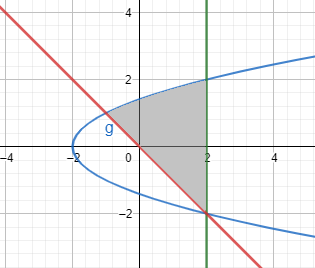
\includegraphics[width=0.2\textwidth]{y^2=x+2,y=-x,x=2.png}
\end{figure}
\item $$ D: y = x^2, y =2+|x| $$\\
Λύση :
\begin{eqnarray*}
I &=& \int _{-2} ^{2} dx \int_{x^2}^{|x|+2} 2xy dy \\
& = & \int_{-2} ^{2}\left[xy^2\right]^{|x|+2}_{x^2} dx \\
& = & \int_{-2} ^{2} (x(|x|+2)^2 - x^5) dx \\
& = & \int_{-2}^{0} x(x^2-2x+4)-x^5dx + \int_{0}^{2} x(x^2+2x+4)-x^5  dx\\
& = & \int_{-2}^{0} x^3-2x^2+4x-x^5dx +\int_{0}^{2} x^3+2x^2+4x-x^5  dx\\
& = & \left[\frac{x^4}{4}-\frac{2}{3}x^3+2x^2-\frac{x^6}{6}\right]^{0}_{-2} + \left[\frac{x^4}{4}+\frac{2}{3}x^3+2x^2-\frac{x^6}{6}\right]^{2}_{0}\\
& = & 0
\end{enumerate}
\begin{figure}[h!]
  \centering
  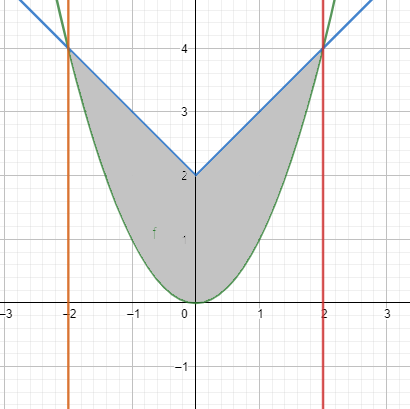
\includegraphics[width=0.2\textwidth]{y=x^2,y=2+x.png}
\end{figure}
\item $$ D: y=-\sqrt{x}, y=-2\sqrt{x}, 1\leq x \leq 4 $$\\
Λύση :
\begin{eqnarray*}
I &=& \int _{1} ^{4} dx \int_{-2\sqrt{x}}^{-\sqrt{x}} (x+2y) dy \\
& = & \int_{1} ^{4}\left[xy+y^2\right]^{-2\sqrt{x}}_{-\sqrt{x}} dx \\
& = & \int_{1} ^{4} (-x\sqrt{x}+x-(-2x\sqrt{x}+(-2\sqrt{x})^2) dx \\
& = & \int_{1}^{4} x\sqrt{x}-3x   dx\\
& = & \int_{1}^{4} x^\frac{3}{2}-3x dx\\
& = & \left[\frac{2}{3}x^\frac{5}{2}\right]_{4}^{1} - \left[\frac{3}{2}x^2\right]_{4}^{1}\\
& = & -\frac{101}{10}
\end{enumerate}
\begin{figure}[h!]
  \centering
  \includegraphics[width=0.2\textwidth]{y=-sqrt{x},y=-2sqrt{x}.png}
\end{figure}
\end{enumerate}
% -----------------------------------------------------
% sixth problem
% -----------------------------------------------------
\item Να υπολογιστούν τα ακόλουθα ολοκληρώματα με χρήση πολικών συντεταγμένων και να σχεδιαστούν τα χωρία ολοκλήρωσης.\selectlanguage {greek}
\begin{enumerate}{}
\item $$ \int\int(x^2+y^2)dxdy \ D:x^2+y^2\leq 4 $$\\
Λύση :
\begin{eqnarray*}
x=pcost, x^2+y^2=p^2, y=psint  , 0\leq p \leq 2, 0\leq t \leq 2\pi \\
I &=& \int\int\frac{θ(x,y)}{θ(p,t)}p^2dpdt\\
& = & \int _{0} ^{2\pi} dt \int_{0}^{2} p^3 dp \\
& = & \int_{0} ^{2\pi}dt \left[\frac{1}{4}p^4\right]_{2}^{0}dp \\
& = & \int_{0} ^{2\pi} 4 dt \\
& = & \left[4t\right]_{0}^{2\pi}\\
& = & 8\pi
\end{enumerate}
\begin{figure}[h!]
  \centering
  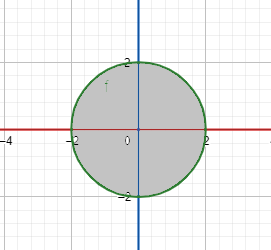
\includegraphics[width=0.2\textwidth]{x^2+y^2,x.png}
\end{figure}
\item $$ \int\int\sqrt{x^2+y^2-9}dxdy \ D:x^2+y^2\leq 25, 9\leq x^2+y^2 $$\\
Λύση :
\begin{eqnarray*}
x=pcost, x^2+y^2=p^2, y=psint  \\
3\leq p \leq 5, 0\leq t \leq 2\pi, \frac{θ(x,y)}{θ(p,t)}=p\\
I &=& \int _{0} ^{2\pi} dt \int_{3}^{5} \frac{θ(x,y)}{θ(p,f)}\sqrt{p^2-9} dp \\
& = & \int_{0}^{2\pi}dt \int_{3}^{5}p\sqrt{p^2-9}dp\\
& = & \frac{1}{2}\frac{2}{3}\int _{0} ^{2\pi} \left[(p^2-9)^\frac{3}{2}\right]_{3}^{5}dt\\
& = & \frac{1}{3} \int_{0}^{2\pi}16^\frac{3}{2}dt\\
& = & \frac{1}{3}\int_{0}^{2\pi}64dt\\
& = & \frac{1}{3}\left[64t\right]_{0}^{2\pi}\\
& = & \frac{128}{3}\pi \\
\end{enumerate}
\begin{figure}[h!]
  \centering
  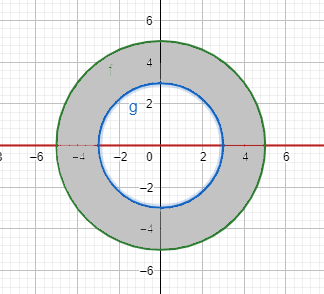
\includegraphics[width=0.2\textwidth]{x^2+y^2,y.png}
\end{figure}
\item $$ \int\int(x+y)dxdy \ D:x^2+y^2\leq 2x $$\\
Λύση :
\begin{eqnarray*}
x=1+pcost, y=psint  ,(x-1)^2+y^2\leq 1 \\
0\leq t \leq 2\pi, \frac{θ(x,y)}{θ(p,t)}=p\\
I &=& \int\int(pcost+1+psint)\frac{θ(x,y)}{θ(p,t)}dpdt\\
& = & \int_{0}^{\2\pi}dt\int_{0}^{1}p+p^2(sint+cost)dt\\
& = & \int_{0}^{2\pi}dt\left[\frac{p^2}{2}+\frac{p^3}{3}(sint+cost)\right]_{0}^{1}\\
& = & \int_{0}^{2\pi}dt(\frac{1}{2}+\frac{1}{3}(sint+cost))\\
& = & \pi + 0\\
& = & \pi\\
\end{enumerate}
\begin{figure}[h!]
  \centering
  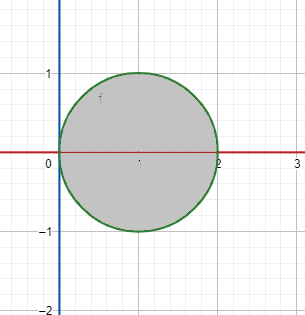
\includegraphics[width=0.2\textwidth]{x^2+y^2,z.png}
\end{figure}
\item $$ \int\int (x+y)dxdy \ D:x^2+y^2\leq x + y $$\\
Λύση :
\begin{eqnarray*}
(x-\frac{1}{2})^2+(y-\frac{1}{2})^2 \leq \frac{1}{2}, p=\sqrt{\frac{1}{2}}\\
x=\frac{1}{2}+psint, \ y=\frac{1}{2} + pcost\\
I &=& \int\int(\frac{1}{2}+pcost+\frac{1}{2}+psint)\frac{θ(x,y)}{θ(p,t)}dpdt\\
& = & \int_{0}^{2\pi}dt\int_{0}^{\frac{1}{\sqrt{2}}}(\frac{1}{2}+pcost+\frac{1}{2}+psint)dp\\
& = & \int_{0}^{2\pi}dt\int_{0}^{\sqrt{2}}p+p^2(cost+sint)dp\\
& = & \int_{0}^{2\pi}\left[\frac{p^2}{2}+\frac{p^3}{3}(cost+sint)\right]_{0}^{\frac{1}{\sqrt{2}}}dt\\
& = & \int_{0}^{2\pi}\left[\frac{1}{4}+\frac{1}{6\sqrt{2}}(cost+sint)\right]dt\\
& = & \frac{\pi}{2}\\
\end{enumerate}
\begin{figure}[h!]
  \centering
  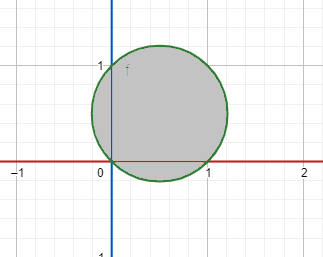
\includegraphics[width=0.2\textwidth]{x^2+y^2,o.png}
\end{figure}
\item $$ \int\int x^2\sqrt{x^2+y^2}dxdy \ D:x^2+y^2\leq 1,x\leq y $$\\
Λύση :
\begin{eqnarray*}
x=pcost, x^2+y^2=p^2, y=psint \\
0\leq p \leq 1, 0\leq t\leq \pi, \frac{θ(x,y)}{θ(p,t)}=p\\
I &=& \int _{0} ^{\pi} dt \int_{0}^{1} \frac{θ(x,y)}{θ(p,t)}\sqrt{p^2}(pcost)^2 dp \\
& = & \int_{0}^{\pi}dt\int_{0}^{1}p^4(cost)^2 dp\\
& = & \int_{0}^{\pi}\frac{(cost)^2}{5}dt \\
& = & \frac{1}{5}\int_{0}^{\pi}\frac{1+cos2t}{2}dt\\
& = & \frac{1}{10}\int_{0}^{\pi}(t+\frac{sin4t}{2})dt\\
& = & \frac{\pi}{10}+\left[\frac{sin2t}{4}\right]_{0}^{\pi}\\
& = & \frac{\pi}{10}\\
\end{enumerate}
\begin{figure}[h!]
  \centering
  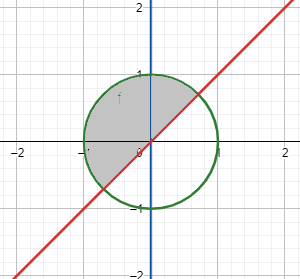
\includegraphics[width=0.2\textwidth]{x^2+y^2,p.png}
\end{figure}
\item $$ \int\int \frac{1}{\sqrt{x^2+y^2}}dxdy \ D:1\leq x^2+y^2 , x^2+y^2\leq 4,x\leq y  $$\\
Λύση :
\begin{eqnarray*}
x=pcost, x^2+y^2=p^2, y=psint \\ 
1\leq p \leq 2, 0\leq t \leq \pi, \frac{θ(x,y)}{θ(p,t)}=p\\
I & = & \int\int\sqrt{t^2}\frac{θ(x,y)}{θ(p,t)}dtdp \\
& = & \int_{0}^{\pi}dt\int_{1}^{2}\frac{1}{\sqrt{p^2}}pdp\\
& = & \int_{0}^{\pi}\left[p\right]_{1}^{2}dt\\
& = & \int_{0}^{\pi}1 dt\\
& = & \left[t\right]_{0}^{\pi} \\
& = & \pi
\end{enumerate}
\begin{figure}[h!]
  \centering
  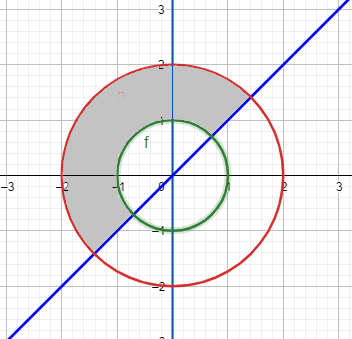
\includegraphics[width=0.2\textwidth]{x^2+y^2,l.png}
\end{figure}
\end{enumerate}
% -----------------------------------------------------
% seventh problem
% -----------------------------------------------------
\item  Νο υπολογιστούν οι όγκοι των ακόλουθων στερεών.\selectlanguage {greek}

\begin{enumerate}{}

\item $$  y = x^2, y = 1, z = 0, z = 2y $$\\
Λύση:
\begin{eqnarray*}
I &=& \int _{-1} ^{1}\int _{x^2} ^{1} dxdy 2y \\
&=&  \int _{-1} ^{1}dx \left[2y \right]^{1}_{x^2} \\
&=&  \int _{-1} ^{1} (1-x^4 )dx \\
&=&  \left[x-\frac{x^5}{5} \right]^{1}_{-1} \\
&=& \frac{8}{5}\\
\end{enumerate}


\item $$ x = 0, y = 0, x + y = 1, z = 0, z = 2xy $$\\
Λύση:
\begin{eqnarray*}
I &=& \int _{0} ^{1}dx\int _{0} ^{1-x}2xy dy  \\
&=&  \int _{0} ^{1}dx \left[xy^2\right]^{1-x}_{0} \\
&=&  \int _{0} ^{1}dx (1-x^2 )^2 \\
&=&  \int _{0} ^{1}dx (x+x^3-2x^2 ) \\
&=&  \left[\frac{x^2}{2}+\frac{x^4}{4}-\frac{2x}{3}\right]^{1}_{0} \\
&=& \frac{1}{12}\\
\end{enumerate}

\item $$ x = 0, y = 1, 2x + y = 5, z = 0, z = xy $$\\
Λύση:
\begin{eqnarray*}
I &=& \int _{0} ^{2}dx\int _{1} ^{5-2x}xy dy  \\
&=&  \int _{0} ^{2}dx \left[x\frac{y^2}{2}\right]^{5-2x}_{1} \\
&=&  \int _{0} ^{2}x (\frac{(5-2x)^2}{2}-\frac{1}{2} )dx \\
&=&  \int _{0} ^{2}x (\frac{25+4x^2-20x}{2}-\frac{1}{2} )dx \\
&=&  \int _{0} ^{2}x (12x+2x^3-10x^2)dx \\
&=&  \left[6x^2+\frac{x^4}{2}-\frac{10x^3}{3}\right]^{2}_{0}  \\
&=& \frac{16}{3}\\
\end{enumerate}


\end{enumerate}


% ---------------------------------------------------
% Anything after the \end{document} will be ignored by the typesetting.
% ----------------------------------------------------

\end{document}

